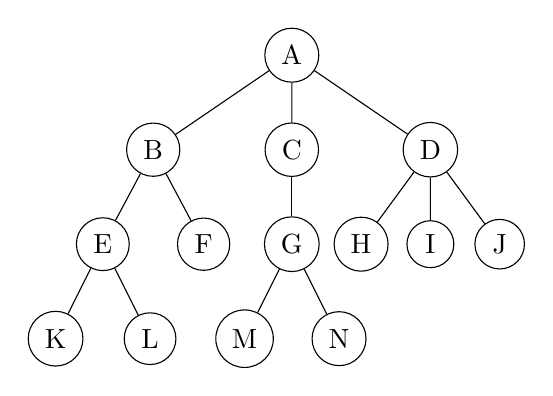
\begin{tikzpicture}[scale=0.8]

  \node [circle,draw] at (0,0) {A}[sibling distance=2.2cm] 
  child { node[circle,draw]{B}[sibling distance=1.6cm]
    child {node[circle,draw]{E}[sibling distance=1.5cm]
      child {node[circle,draw]{K}}
      child {node[circle,draw]{L}}
    }
    child {node[circle,draw]{F}}      
  }    
  child { node[circle,draw]{C}
    child {node[circle,draw]{G}[sibling distance=1.5cm]          
      child {node[circle,draw]{M}} 
      child {node[circle,draw]{N}}   
    }			
  }	
  child { node[circle,draw]{D}[sibling distance=1.1cm]
    child {node[circle,draw]{H}} 
    child {node[circle,draw]{I}}
    child {node[circle,draw]{J}}
  };  
\end{tikzpicture}
